\chapter{Estudo de Caso}
\label{cap:proposta}

Nos capítulos anteriores foram apresentas algumas tecnologias importantes para a implementação de aplicações que se encaixam no contexto Big Data. O propósito desta etapa inicial consistiu em levantar o conhecimento necessário para que seja possível analisar e projetar soluções baseadas em diferentes cenários que envolvem o processamento de grandes volumes de dados. Nesta fase do projeto, o objetivo consiste em aplicar os conceitos vistos até o momento em um estudo de caso real. Portanto, ao longo deste capítulo descreve-se um modelo de arquitetura que será construído para simular um ambiente nesses moldes, onde seja necessário manipular e analisar uma grande quantidade de dados, além de prover escalabilidade linear.

\section{Motivação}

Com o surgimento de políticas públicas voltadas para transparência digital, principalmente após o estabelecimento da Lei de Acesso à Informação\footnote{\url{http://www.planalto.gov.br/ccivil_03/_ato2011-2014/2011/lei/l12527.htm}}, a população brasileira tem exercido um papel fundamental no monitoramento das atividades exercidas por seus representantes. A realização de eventos como a maratona Hackathon\footnote{\url{http://www2.camara.leg.br/responsabilidade-social/edulegislativa/educacao-legislativa-1/educacao-para-a-democracia-1/hackathon/hackathon}} da Câmara dos Deputados contribui e incentiva ainda mais a adesão da comunidade de desenvolvedores para a construção de softwares voltados para este contexto.

As redes sociais também desempenham uma função essencial nesse processo. Este meio de comunicação deixou de ser utilizado apenas como lazer e atualmente é usado pelos cidadãos para expressar opiniões sobre os mais variados assuntos, princialmente quando refere-se a questões políticas e sociais aplicadas no país.

\section{Problema}

A política brasileira vem sendo bastante criticada nos últimos anos, escândalos políticos, notícias frequentes sobre corrupção, serviços públicos de má qualidade, entre outros fatores, contribuem para a insatisfação do cidadão brasileiro em relação ao governo do país. Tendo em vista que as redes sociais são utilizadas por grande parcela da população como meio para expressar suas opiniões, uma análise minuciosa destas informações pode ser um fator de extrema importância para compreender a percepção das pessoas sobre seus representantes. Processar estas informações não é uma tarefa trivial, pois os dados gerados por este meio podem estar na ordem de terabytes.

\section{Arquitetura}

Nesta seção, será apresentado um modelo para solucionar o problema descrito anteriormente. A quantidade de dados gerados por redes sociais exige uma abordagem voltada para o contexto Big Data, pois, como mostrado nos capítulos anteriores, bancos de dados relacionais e outras tecnologias tradicionais não são adequadas a esse cenário. Portanto, o estudo de caso proposto por este trabalho tem como objetivo a construção de uma aplicação que realize análise de dados de redes sociais, buscando publicações que citem os candidatos que concorreram às eleições do segundo turno para Presidência da República no ano de 2014. As mensagens capturadas devem expressar opiniões sobre estes políticos, permitindo investigar a percepção dos internautas antes, durante e após o período correspondente às eleições. A figura \ref{fig-arq-projeto} ilustra a arquitetura proposta.

\begin{figure}[ht!]
	\centering
	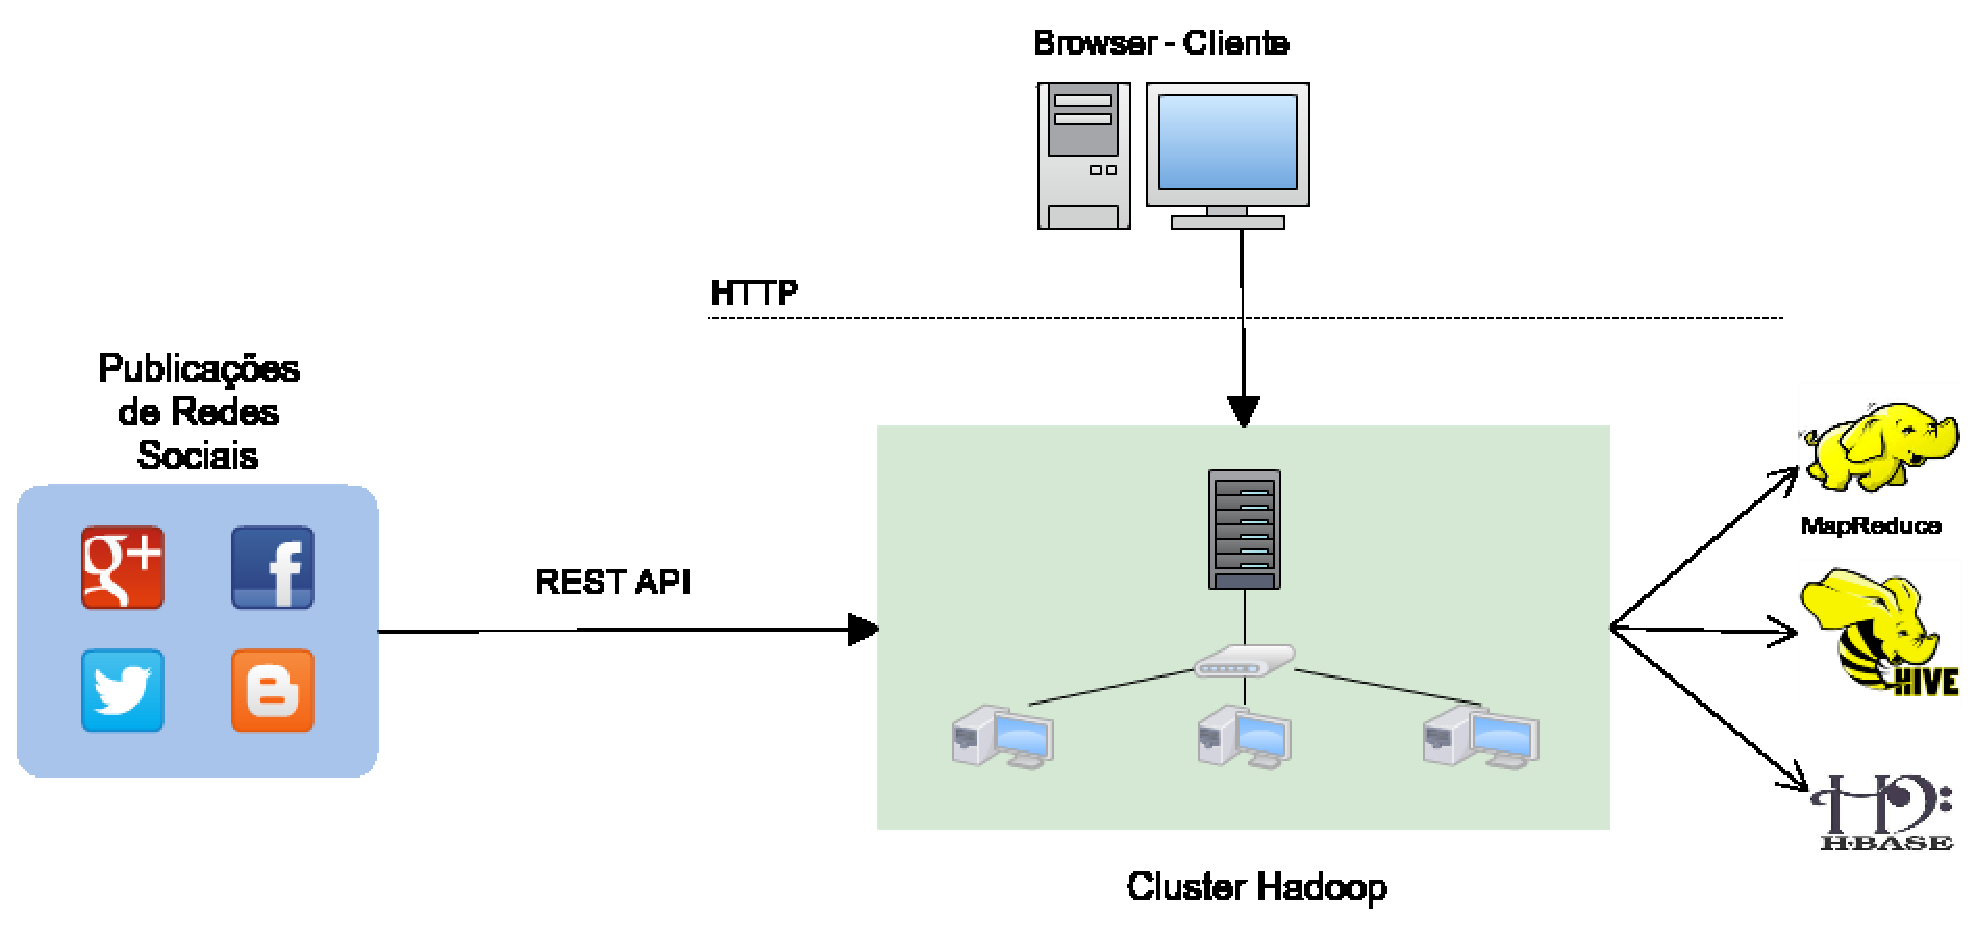
\includegraphics[keepaspectratio=true,scale=0.35]
	  {figuras/arquitetura.eps}
	\caption[Arquitetura proposta]{Arquitetura proposta
	\protect\linebreak Fonte: Autor}
	\label{fig-arq-projeto}
\end{figure}
\FloatBarrier

A arquitetura apresentada na figura \ref{fig-arq-projeto} é composta, principalmente, por um \textit{cluster} Hadoop, o qual é responsável por receber e armazenar as mensagens coletadas do Facebook e Twitter, as redes sociais escolhidas como fonte de informações para este trabalho. A captura de publicações é feita utilizando APIs baseadas no protocolo REST\footnote{\url{http://pt.wikipedia.org/wiki/REST}}, que serão detalhadas nas próximas seções. Os dados resididos no \textit{cluster} são processados e os resultados são exportados para um banco de dados relacional MySQL. A transição entre estes dois ambientes ocorre com o auxílio da ferramenta Sqoop. Por fim, uma interface \textit{web}, construída utilizando a linguagem Java, disponibiliza os resultados finais da etapa de análise. A figura \ref{fig-atividades} apresenta um fluxo com as principais atividades envolvidas neste estudo de caso.

\begin{figure}[ht!]
	\centering
	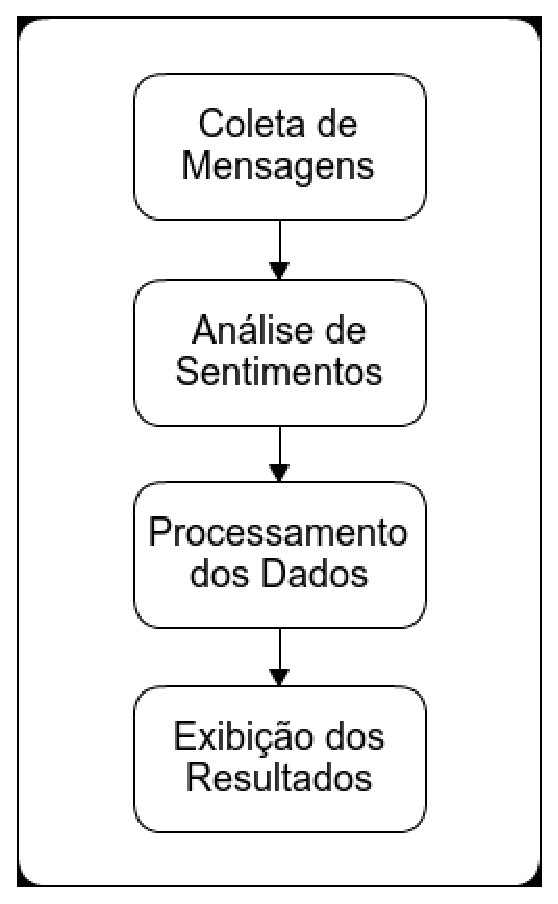
\includegraphics[keepaspectratio=true,scale=0.5]
	  {figuras/atividades.eps}
	\caption[Atividades envolvidas no estudo de caso]{Atividades envolvidas no estudo de caso
	\protect\linebreak Fonte: Autor}
	\label{fig-atividades}
\end{figure}
\FloatBarrier

A seguir, é apresentada uma breve descrição sobre as atividades ilustradas na figura \ref{fig-atividades}:

\begin{itemize}

  \item \textbf{Coleta de Mensagens:} Consiste na busca por mensagens publicadas no Facebook e Twitter, onde se utilizam as APIs disponibilizadas por estas redes sociais, as quais são voltadas aos desenvolvedores de aplicações. Nesta etapa, são pesquisadas mensagens que citam os dois candidatos à Presidência da República durante o segundo turno das eleições de 2014. Para este trabalho, foram coletadas publicações realizadas entre janeiro de 2014 e abril de 2015. A ingestão destes dados no \textit{cluster} é realizada com o auxílio da ferramenta Flume, a qual exige uma implementação personalizada que será abordada na seção \ref{sec:coleta-imp}.
  \item \textbf{Análise de Sentimentos:} As mensagens coletadas passam por um processo de análise de sentimentos, onde são classificadas de acordo com o sentimento expresso pelo autor de cada publicação a respeito de um determinado candidato. Desta forma, é possível realizar uma breve análise sobre a percepção de uma parcela de usuários sobre estas personalidades públicas.
  \item \textbf{Processamento dos Dados:} Concluídas as etapas anteriores, todas as mensagens resididas no \textit{cluster} são processadas e agrupadas com auxílio da ferramenta de \textit{data warehouse} Hive, a qual permite obter resultados gerais sobre a fase de análise de sentimentos das mensagens de cada candidato. Estes resultados são exportados para o banco de dados relacional MySQL através da ferramenta Sqoop.
  \item \textbf{Exibição dos Resultados:} Com os resultados já persistidos no banco relacional, uma interface \textit{web} permite a visualização destas informações finais, disponibilizando gráficos e tabelas com os resultados do processo de análise de sentimentos para cada um dos candidatos analisados.

\end{itemize}

As seções seguintes descrevem estas atividades com um maior nível de detalhamento, especificando todos os componentes da arquitetura proposta por este estudo de caso. O \textit{cluster} utilizado neste trabalho, juntamente com as outras ferramentas necessárias, foram configurados em uma única máquina com sistema operacional Ubuntu 12.04. O código fonte das implementações e os arquivos de configuração utilizados estão disponíveis no diretório \textit{implementacao}, localizado no seguinte repositório da ferramenta Github\footnote{\url{https://github.com/}}: \url{https://github.com/guilhermedelima/tcc}.

\section{Coleta de Mensagens}
\label{sec:coleta-imp}

Nesta seção, são ilustrados os passos necessários para a conclusão da etapa referente a coleta de mensagens. Inicialmente, é apresentada uma breve explicação sobre as APIs do Facebook e Twitter e a definição da metodologia utilizada para pesquisar as publicações. Por fim, apresenta-se o Flume e a implementação construída para capturar as mensagens e armazená-las no \textit{cluster}.

\subsection{Facebook}

Uma das redes sociais de maior sucesso atualmente, o Facebook conta com uma média superior a 890 milhões de usuários diários ativos \cite{facebook-doc}. Além de ser um veículo utilizado para interação entre pessoas, também é comum o seu uso para exposição de opiniões e preferências políticas, religiosas, entre uma infinidade de temas. Devido à sua expressividade, tornou-se comum a utilização do Facebook por pessoas públicas, como políticos e celebridades, seja para divulgação de notícias e informações imparciais, como também para exposição de ideias e opiniões pessoais. Determinadas páginas possuem, inclusive, um selo identificando sua autenticidade, confirmando a utilização daquele meio pela personalidade pública em questão.

Pelas características apresentadas, o Facebook se torna uma fonte de informações indispensável para busca de opiniões. A principal forma de obter dados desta rede social é através da chamada \textit{Graph} API\footnote{\url{https://developers.facebook.com/docs/graph-api}}, uma plataforma HTTP de baixo nível que permite não apenas consultas, mas também publicar postagens, gerenciar contatos, divulgar fotos, e uma variedade de funcionalidades. O nome desta API deriva da ideia de um grafo social, onde os vértices são representados por pessoas, fotos, comentários, etc., já arestas expressam a conexão entre esses elementos.

Um dos objetivos deste trabalho é retirar postagens onde pessoas externam opiniões pessoais sobre os candidatos citados anteriormente. A principal forma de um usuário manisfestar estas informações é através de postagens em sua linha do tempo, onde cria-se um tópico específico permitindo, inclusive, respostas de amigos e pessoas autorizadas. A versão 1.0 da \textit{Graph} API possibilitava a busca por postagens públicas, entretanto, por motivos não revelados, esta funcionalidade foi descontinuada pela equipe do Facebook, não sendo possível executá-la.

Outra forma na qual usuários podem interagir consiste na postagem em páginas de pessoas públicas, empresas, entre outros. Apesar da semelhança com a linha do tempo de um usuário comum, estas páginas possuem um caráter integralmente público, onde qualquer indivíduo tem permissão para ler e escrever postagens. Nestes locais, é possível identificar comentários onde usuários expressam opiniões e participam de discussões. Para contornar as limitações descritas no parágrafo anterior e realizar a coleta dos dados, optou-se por buscar todos os comentários publicados nas páginas oficiais de cada candidato analisado. Portanto, todas as postagens retiradas do Facebook são oriundas, exclusivamente, das páginas públicas e autenticadas. A tabela \ref{tab-fb-pags} apresenta as páginas utilizadas para coleta das mensagens.	

\begin{table}[!ht]
\begin{center}
  \begin{tabular}{|p{5cm}|p{5cm}|}
	\hline
	Candidato & Página no Facebook
	\\ \hline
	Aécio Neves & AecioNevesOficial
	\\ \hline
	Dilma Rousseff & SiteDilmaRousseff
	\\ \hline
  \end{tabular}
  \captionsetup{justification=centering}
  \caption[Páginas utilizadas para pesquisa]{Páginas utilizadas para pesquisa
  \protect\linebreak Fonte: Autor}
\label{tab-fb-pags}
\end{center}
\end{table}
\FloatBarrier

Como mencionado anteriormente, a \textit{Graph} API é baseada apenas no protocolo HTTP. Uma das funcionalidades presentes nesta arquitetura é a busca por páginas do Facebook, para isso basta montar uma requisição informando o \textit{id} de uma determinada página. O resultado desta solicitação será um objeto JSON\footnote{Acrônimo para JavaScript \textit{Object Notation}. Especifica um formato leve para transferência de dados computacionais, derivado de um subconjunto da notação de objeto da linguagem JavaScript.} contendo todos os campos do elemento requerido, neste caso, a própria página. A tabela \ref{tab-fb-campos} apresenta alguns destes campos.

\begin{table}[!ht]
\begin{center}
  \begin{tabular}{|p{5cm}|p{7cm}|}
	\hline
	Campo & Descrição
	\\ \hline
	\textit{id} &  Inteiro que identifica a página.
	\\ \hline
	\textit{about} & Informação da página.
	\\ \hline
	\textit{category} & Categoria da página, por exemplo, tecnologia, política e serviços.
	\\ \hline
	\textit{name} & Nome da página.
	\\ \hline
	\textit{likes} & Número de usuários que curtiram a página.
	\\ \hline
  \end{tabular}
  \captionsetup{justification=centering}
  \caption[Campos de uma página pública do Facebook]{Campos de uma página pública do Facebook
  \protect\linebreak Fonte: Adaptado de \cite{facebook-page-doc}}
\label{tab-fb-campos}
\end{center}
\end{table}
\FloatBarrier

Uma página representa um vértice do grafo social montado pelo Facebook, assim como as postagens, fotos, álbuns, notificações e outros elementos que estão relacionados a mesma. Para obter as publicações efetuadas em uma página é necessário acrescentar à requisição o nome da aresta que faz a ligação entre eles. A figura \ref{facebook-rest} apresenta como seria uma requisição HTTP para consultar as publicações de uma página qualquer.

\begin{figure}[ht!]
	\centering
	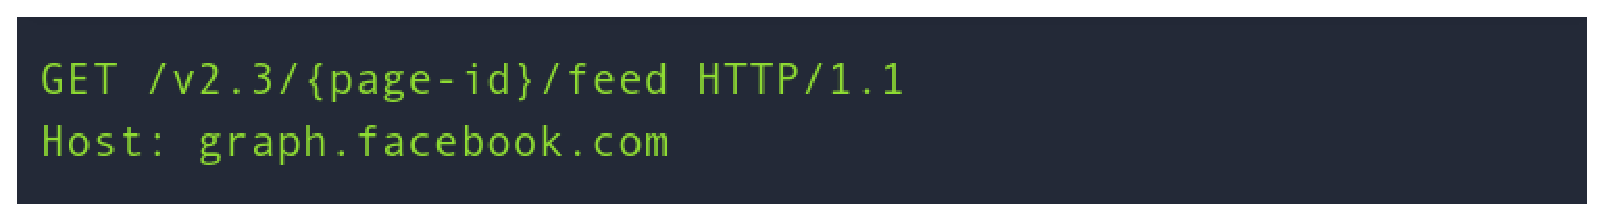
\includegraphics[keepaspectratio=true,scale=0.35]
	  {figuras/fb-http.eps}
	\caption[Requisição HTTP para obter publicações de páginas do Facebook]{Requisição HTTP para obter publicações de páginas do Facebook
	\protect\linebreak Fonte: \cite{facebook-page-doc}}
	\label{facebook-rest}
\end{figure}
\FloatBarrier

O resultado da requisição ilustrada na figura \ref{facebook-rest} também será um objeto JSON com diversos campos, incluindo os comentários públicos efetuados por usuários. Através dos comentários, é possível identificar o autor, data da postagem e o corpo da mensagem. O Facebook utiliza o protocolo \textit{OAuth}\footnote{\url{http://en.wikipedia.org/wiki/OAuth}} para autorizar o uso dos recursos da \textit{Graph} API, portanto, todas as requisições submetidas devem utilizar um \textit{access token}, que pode ser obtido na página voltada aos desenvolvedores de aplicações.

\subsection{Twitter}

Outra rede social em evidência no cenário atual, o Twitter apresenta um número superior a 280 milhões de usuários ativos mensais, além de uma média equivalente a 500 milhões de mensagens publicadas por dia \cite{twitter-doc}. O modelo adotado pelo Twitter tem uma complexidade bem menor, quando comparado ao Facebook, seu proposito consiste em oferecer um microblog onde usuários podem publicar mensagens de no máximo 140 caracteres, conhecidas como \textit{tweets}.

Para coletar \textit{tweets} com opiniões de usuários, optou-se por realizar uma busca por mensagens utilizando filtragem textual e temporal. Ao contrário do Facebook, o Twitter autoriza pesquisas por comentários públicos em páginas pessoais, portanto, o recolhimento dos \textit{tweets} se torna uma atividade mais acessível. A tabela \ref{tab-tw-nomes} apresenta os termos usados para pesquisar as publicações que expressam opiniões, ou simplesmente citam os candidatos analisados neste trabalho.

\begin{table}[!ht]
\begin{center}
  \begin{tabular}{|p{5cm}|p{5cm}|}
	\hline
	Candidato & Termos utilizados
	\\ \hline
	Aécio Neves & aecio, aecio neves
	\\ \hline
	Dilma Rousseff & dilma, dilma rousseff
	\\ \hline
  \end{tabular}
  \captionsetup{justification=centering}
  \caption[Termos adotados para pesquisa dos candidatos no Twitter]{Termos adotados para pesquisa dos candidatos no Twitter
  \protect\linebreak Fonte: Autor}
\label{tab-tw-nomes}
\end{center}
\end{table}
\FloatBarrier

O Twitter permite a extração de publicações através de duas formas distintas. A primeira maneira se dá pelo uso da \textit{Search} API\footnote{\url{https://dev.twitter.com/rest/public/search}}, um componente da REST API\footnote{\url{https://dev.twitter.com/rest/public}}, a qual possibilita execução de consultas HTTP para obter os \textit{tweets} mais recentes e relevantes. Apesar da semelhança com a ferramenta de busca padrão, disponível para os usuários do Twitter, esta API apresenta algumas limitações, entre elas, o número de \textit{tweets} que podem ser adquiridos. Utilizando a \textit{Search} API, é possível obter apenas as mensagens publicadas entre os últimos 6 ou 9 dias, postagens antigas não são indexadas pela API. Também há um limite de 180 requisições realizadas a cada 15 minutos, ao exceder este valor, as solicitações são negadas até o recomeço de uma nova janela de transmissão.

Outra forma de consultar as publicações do Twitter é através da \textit{Streaming} API\footnote{\url{https://dev.twitter.com/streaming/overview}}, um módulo que possibilita a captura de mensagens publicadas em tempo real. Diferente da \textit{Search} API, este modelo mantém uma conexão aberta em um processo separado, o qual notifica o programa principal ao receber novos dados. Desta maneira, o servidor não é inundado com requisições, oferecendo uma opção leve para a coleta de mensagens em tempo real.

Semelhante ao Facebook, o Twitter também utiliza o protocolo \textit{OAuth} para autorizar as requisições HTTP que desejam acessar os serviços da rede social, portanto, é necessário obter um \textit{access token} na área voltada aos desenvolvedores do microblog. Ambas as APIs de busca oferecidas retornam as requisições em objetos no formato JSON, onde é possível identificar o autor do comentário, a data de publicação, o texto da mensagem, entre outros campos.

\subsection{Apache Flume}

Assim como discutido em seções anteriores, um dos grandes desafios inerentes ao uso de tecnologias Big Data se dá pela dificuldade na manipulação de quantidades elevadas de informações. A solução apresentada pelo Hadoop para o armazenamento em larga escala envolve algumas questões técnicas que o diferenciam dos diversos paradigmas tradicionais presentes na computação. Segundo \citeonline{hoffmanFlume}, em sistemas de arquivos POSIX, durante uma operação de escrita os dados inseridos se mantém persistidos no disco antes mesmo do fechamento do arquivo e término de todo procedimento. Isto significa que se outro processo realizar operações de leitura, ele será capaz de ler os dados que estão sendo escritos no momento. Caso ocorra uma interrupção durante um processo de escrita, as informações registradas até o momento continuam no arquivo, de maneira incompleta, porém parcialmente visíveis.

Por outro lado, o HDFS apresenta um modelo dissimilar. Arquivos escritos neste sistema de arquivos distribuídos são interpretados como uma entrada de diretório de tamanho nulo até o período em que a operação é finalizada. Portanto, caso um processo cliente realize alguma operação de escrita de longa duração, e por alguma razão não a conclua, ao término deste cenário o usuário terá acesso apenas a um arquivo vazio.

Realizar a escrita de arquivos pequenos pode parecer uma alternativa para este problema, pois desta forma, as operações são finalizadas rapidamente, e consequentemente reduziria a probabilidade de perdas durante o processo. Entretanto, esta estratégia resulta em considerável perda de performance do HDFS. Segundo \citeonline{white2012}, cada arquivo, diretório ou bloco representa um objeto na memória do \textit{namenode} do \textit{cluster}, ocupando 150 bytes cada. Além do desperdício de memória, a execução de \textit{MapReduce} \textit{jobs} seria menos eficiente, pois arquivos pequenos representam blocos de tamanhos reduzidos, ocasionando \textit{input splits} reduzidos. Desta forma, seria necessário um número maior de \textit{map tasks}, o que impacta em um maior tempo de execução.

Inserido nesse contexto, o Apache Flume é um projeto com objetivo de oferecer suporte para situações onde é necessário realizar transferência de registros de uma determinada fonte de dados para um destino final, como HDFS. O Flume foi criado para ser uma ferramenta padronizada, simples, robusta e flexível para ingestão de dados dentro do Hadoop \cite{hoffmanFlume}. Sua arquitetura é composta por três módulos principais: \textit{source}, \textit{channel} e \textit{sink}. A figura \ref{flume-arch} apresenta este modelo.

\begin{figure}[ht!]
	\centering
	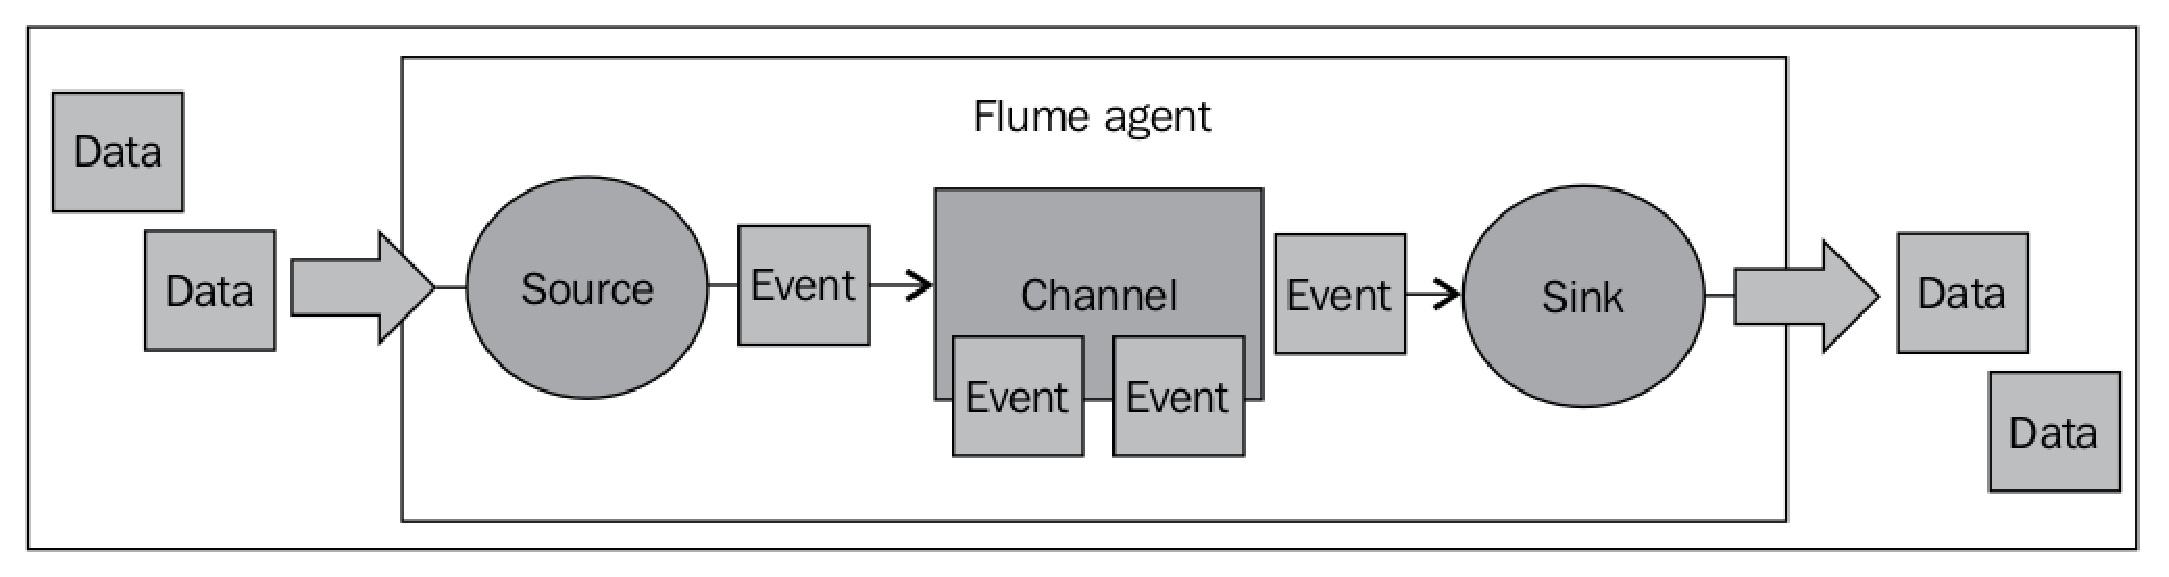
\includegraphics[keepaspectratio=true,scale=0.4]
	  {figuras/flume.eps}
	\caption[Arquitetura Flume]{Arquitetura Flume
	\protect\linebreak Fonte: Retirado de \cite{hoffmanFlume}}
	\label{flume-arch}
\end{figure}
\FloatBarrier

O agente Flume apresentado na figura \ref{flume-arch} representa o processo executado pela ferramenta, o qual realiza todo procedimento de transferência de informações entre os dois ambientes. Um \textit{source} é uma \textit{thread} responsável por capturar os dados de uma determinada fonte, geralmente um serviço que caracteriza-se por produzir dados a todo instante, como registros de log, publicações de redes sociais, ou similares. Os dados coletados pelo \textit{source} são convertidos para um formato específico do Flume, denominado evento, o qual é composto apenas por um cabeçalho e o conteúdo da mensagem.

Todos os eventos criados por um \textit{source} são escritos em uma área de espera chamada \textit{channel}, responsável pela ligação entre \textit{sources} e \textit{sinks}. Um \textit{channel} representa um \textit{buffer}, podendo armazenar seus dados em memória, ou também em arquivos. Segundo \citeonline{hoffmanFlume}, o uso de arquivos permite que um \textit{channel}, antes de disponibilizar os eventos para leitura, efetue todas as alterações no sistema de arquivos local, oferecendo maior espaço físico e tolerância a falhas. Por outro lado, \textit{channels} baseados em memória, apesar da escassez de recursos e volatilidade dos dados, possuem performance superior.

O \textit{sink} representa o último componente do modelo proposto pelo Flume. Sua execução ocorre em uma \textit{thread} independente, com responsabilidade de coletar eventos disponibilizados por um \textit{channel} e transferir estes dados para uma fonte de destino, geralmente o HDFS. O trabalho de um HDFS \textit{sink} é, continuamente, abrir um arquivo no HDFS, transferir dados para ele, e em algum momento fechá-lo e iniciar um novo \cite{hoffmanFlume}.

Com esta arquitetura, é possível criar fluxos complexos e variados, adaptando-se a diferentes cenários. A combinação de \textit{sources}, \textit{channels} e \textit{sinks} tornam o Flume uma ferramenta poderosa para ingestão de dados no HDFS.

\subsection{Implementação Flume}

Para coletar as mensagens das fontes de informações disponíveis, foi necessário a implementação de três \textit{sources} distintos, de acordo com as redes sociais selecionadas e suas APIs de acesso.

\begin{itemize}

  \item \textbf{Facebook:} utiliza a \textit{Graph} API para obter os comentários das páginas oficiais dos candidatos.
  \item \textbf{Twitter Rest:} faz uso da \textit{Search} API para coletar os \textit{tweets} publicados entre os últimos 6 ou 9 dias.
  \item \textbf{Twitter \textit{Streaming}:} captura os \textit{tweets} em tempo real utilizando a \textit{Streaming} API.

\end{itemize}

A figura \ref{flume-imp} ilustra o fluxo da informação durante todo o processo de coleta de mensagens, iniciando na interação com as APIs das redes sociais, passando pelos componentes do Flume e finalizando com as postagens armazenadas no HDFS.

\begin{figure}[ht!]
	\centering
	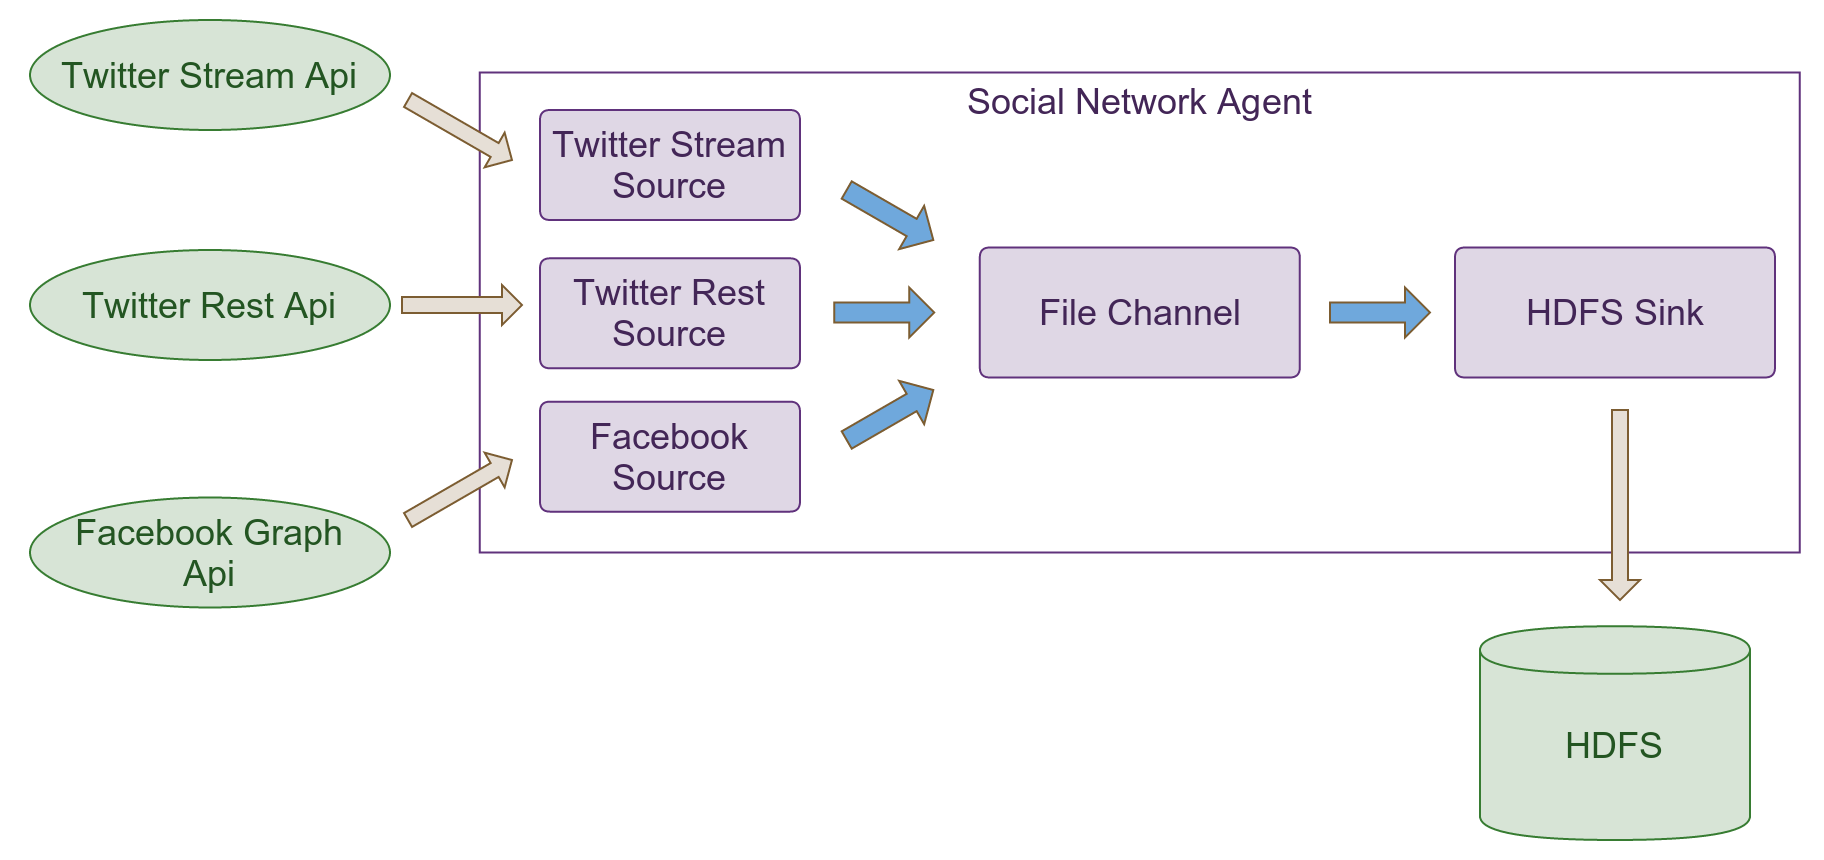
\includegraphics[keepaspectratio=true,scale=0.2]
	  {figuras/flume-imp.eps}
	\caption[Arquitetura da coleta de mensagens.]{Arquitetura da coleta de mensagens.
	\protect\linebreak Fonte: Autor}
	\label{flume-imp}
\end{figure}
\FloatBarrier

O bloco denominado \textit{Social Network Agent} representa todo o processo que será executado no Flume. Cada \textit{source} diferente, na prática, simboliza uma classe customizada que estende a classe \textit{AbstractSource} e implementa as interfaces \textit{EventDrivenSource} e \textit{Configurable}, pertencentes a API do Flume. A interação destes componentes com as APIs das redes sociais ocorre com o uso das bibliotecas Facebook4j\footnote{\url{http://facebook4j.org/}} e Twitter4j\footnote{\url{http://twitter4j.org/}}, encapsulando o uso do protocolo REST para facilitar a fase de desenvolvimento.

A imagem \ref{flume-uml} apresenta uma arquitetura simplificada dos elementos responsáveis por realizar a captura de mensagens. O pacote \textit{Source} é composto pelas classes que implementam diretamente \textit{sources} do Flume, onde utilizam serviços do pacote \textit{Service}, responsável por se comunicar diretamente com as redes sociais.

\begin{figure}[ht!]
	\centering
	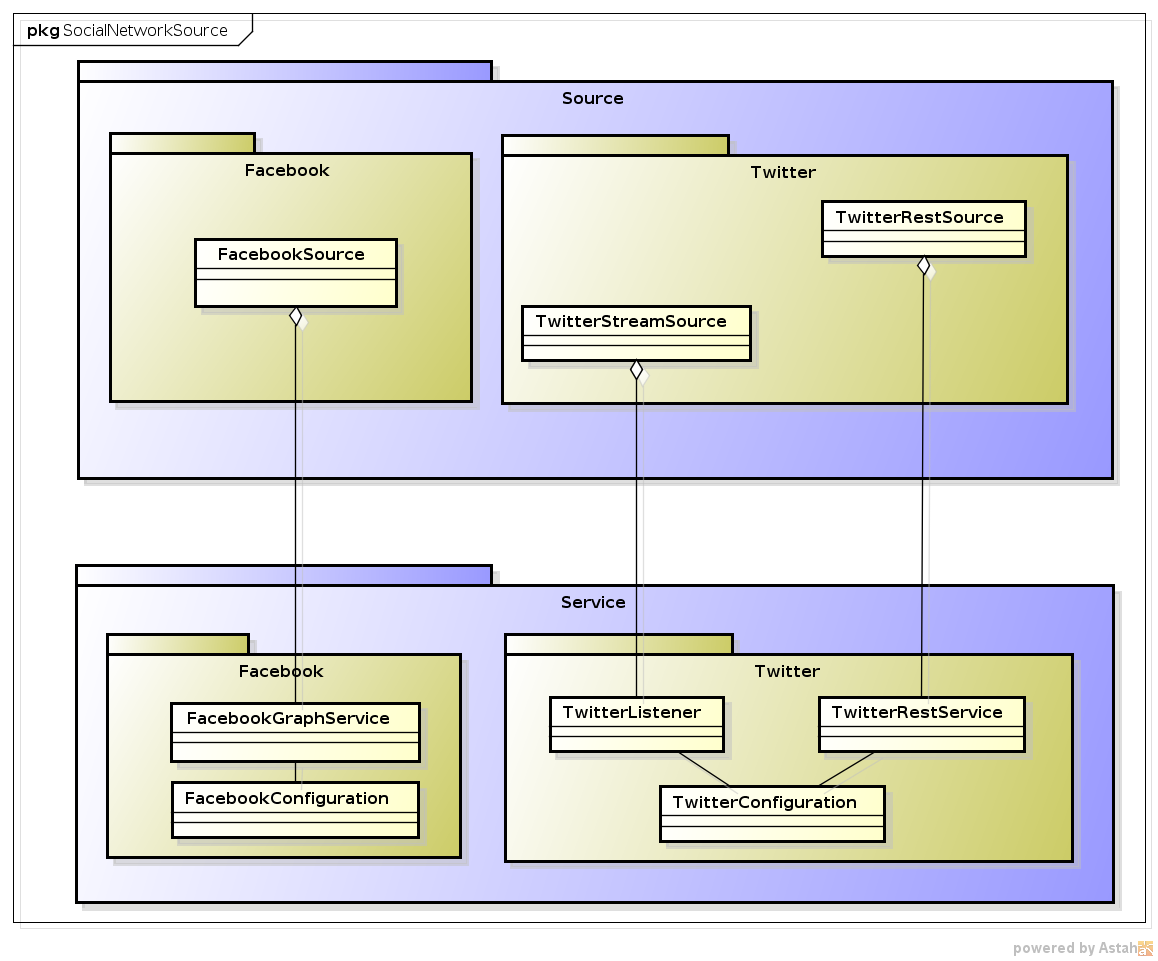
\includegraphics[keepaspectratio=true,scale=0.5]
	  {figuras/flume-uml.eps}
	\caption[Arquitetura dos \textit{sources} customizados]{Arquitetura dos \textit{sources} customizados
	\protect\linebreak Fonte: Autor}
	\label{flume-uml}
\end{figure}
\FloatBarrier

Ainda na figura \ref{flume-uml}, é possível perceber que os eventos gerados pelos diferentes \textit{sources} são escritos em um único \textit{file channel}, o qual conta com um arquivo no próprio disco local para armazenamento temporário. Desta forma, evita-se que na ocorrência de falhas todo o progresso até o momento seja perdido.

Cada evento gerado é composto por um objeto JSON com as informações a respeito da mensagem coletada. Após estarem disponíveis no \textit{file channel}, o HDFS \textit{sink} se encarrega de abrir arquivos no HDFS e transferir os eventos do \textit{buffer} para o \textit{cluster}. A maneira como este \textit{sink} copia os eventos para um arquivo no HDFS pode ser ajustada através de parâmetros presentes no arquivo de configuração do Flume. É importante garantir uma vazão alta juntamente com a criação de arquivos grandes no HDFS. Segundo \citeonline{white2012}, o uso de arquivos pequenos prejudica consideravelmente o desempenho de \textit{MapReduce} \textit{jobs}, além do uso excessivo de memória pelo \textit{namenode}, pois cada arquivo, diretório e bloco representa um objeto de 150 bytes.

\section{Análise de Sentimentos}

As seções anteriores apresentaram a metodologia utilizada para realizar a coleta das mensagens provenientes do Facebook e Twitter. Nesta fase, será relatado o paradigma adotado para efetuar a análise de sentimentos sobre as publicações armazenadas no HDFS. O objetivo desta etapa é a definição de um modelo, onde mensagens de um candidato específico devem ser processadas e classificadas em dois grupos distintos: postagens que expressam sentimentos positivos ou negativos a respeito do indivíduo.

Uma abordagem comum para análise de sentimentos é a classificação do texto através do emprego de recursos léxicos, onde utiliza-se uma base constituída de termos opinativos previamente computados. O SentiWordNet é um dos métodos mais conhecidos que implementam este modelo, segundo \citeonline{araujo2013}, este classificador usa o dicionário léxico \textit{WordNet} como parâmetro para, posteriormente, atribuir a cada palavra uma pontuação variando de 0 a 1, atribuindo estes valores para cada um dos sentimentos possíveis: negativo, neutro e positivo.

O uso da análise léxica apresenta algumas desvantagens significativas. Sua utilização é dependente, primeiramente, da existência de uma base previamente classificada e disponível para o idioma adotado. O uso de termos pré computados também pode afetar a classificação de uma sentença, pois algumas palavras, quando inseridas em contextos diferentes, podem representar sentimentos opostos. Por estas razões, optou-se por utilizar um método baseado em aprendizado de máquina, livre de restrições relativas a dicionários já existentes.

O classificador \textit{Naive Bayes} pode ser considerado um dos principais métodos conhecidos para problemas relacionados a aprendizagem de máquina. Segundo pesquisa realizada por \citeonline{mitchell_1997}, esta abordagem, para muitos casos, apresenta um nível de confiabilidade semelhante a outros algoritmos complexos, como árvores de decisão e redes neurais. Este modelo faz uso de fórmulas estatísticas e cálculos de probabilidade para realizar a classificação. Através do Teorema de \textit{Bayes}, o classificador calcula a probabilidade de uma evidência $E = e_{1}, e_{2} … e_{n}$ pertencer a uma classe de acordo com a seguinte fórmula.

\begin{equation}
P(classe | E) = \frac{P(e_{1} ... e_{n} | classe) \times P(classe)}{P(e_{1} ... e_{n})}
\end{equation}

Para definir a classe mais provável de uma evidência, calcula-se a probabilidade de todas as classes existentes, para em seguida, escolher a classe com a probabilidade mais alta de ocorrência. Em termos estatísticos, isso é análogo a maximizar o valor de $P(classe | E)$. O cálculo de $P(e_{1} … e_{n} | classe)$ torna-se complexo de ser obtido, pois possivelmente não há uma ocorrência similar presente na base de treinamento. Para este cenário, o classificador \textit{Naive Bayes} realiza uma simplificação, onde “ingenuamente” considera que as evidências são fatores independentes. Portanto, o cálculo é reduzido ao produto das probabilidades de cada evidência individual. Aplicando estas observações e eliminando a constante $P(e_{1} … e_{n})$, a fórmula pode ser reduzida, como apresentada a seguir.

\begin{equation}
arg\;max\;P(classe | E) = \prod_{i=1}^{n} P(e_{i} | classe) \times P(classe)
\end{equation}

Apesar de ser possível perceber que a afirmação, na qual as evidências são atributos independentes, é falsa na maioria das vezes, segundo \citeonline{mitchell_1997}, o classificador \textit{Naive Bayes}, mesmo assim, é capaz de produzir resultados consideravelmente satisfatórios. Por estas razões, optou-se por utilizar este método para classificar os comentários coletados nas redes sociais.

Para cada um dos candidatos analisados, foi construída uma base de treinamento independente, com aproximadamente 300 publicações retiradas do Facebook e Twitter, onde cada comentário foi classificado de acordo com o sentimento expresso pelo autor, pertencendo a classe \textbf{positivo} ou \textbf{negativo}. Após a fase de elaboração das bases de treinamento, iniciou-se a etapa de coleta e classificação das mensagens. A figura \ref{senti-analysis} apresenta as atividades executadas durante este processo.

\begin{figure}[ht!]
	\centering
	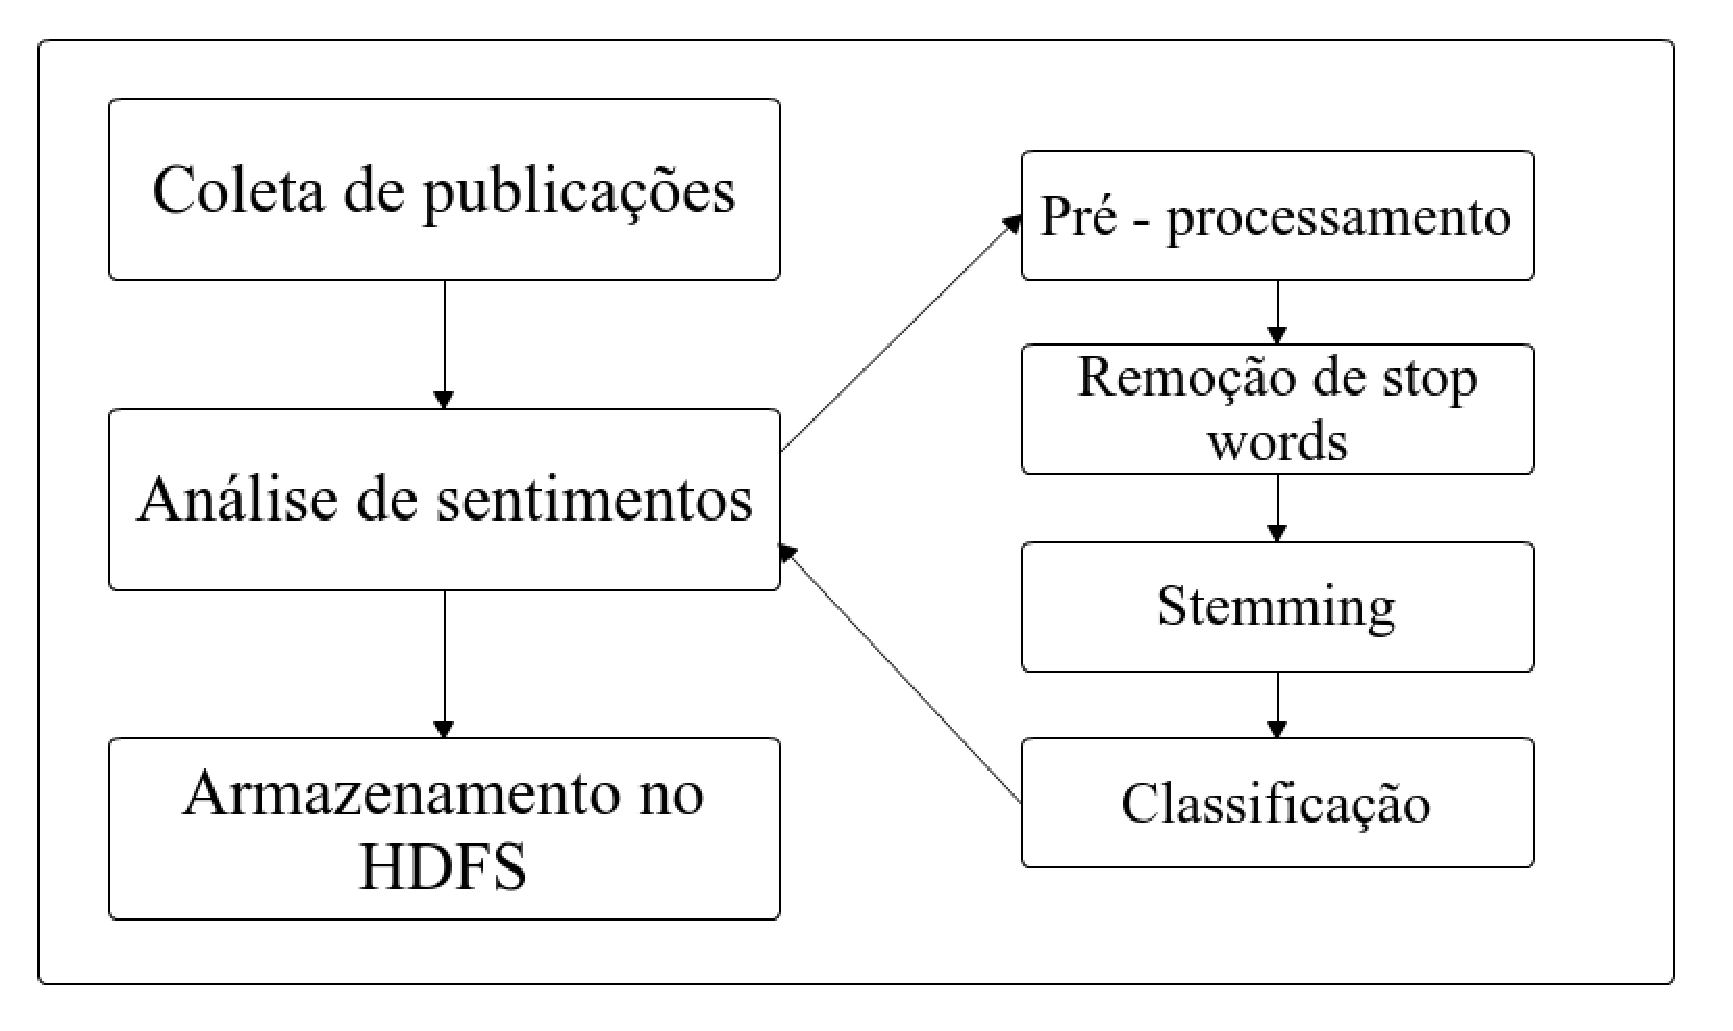
\includegraphics[keepaspectratio=true,scale=0.4]
	  {figuras/as.eps}
	\caption[Processo de análise de sentimentos]{Processo de análise de sentimentos
	\protect\linebreak Fonte: Autor}
	\label{senti-analysis}
\end{figure}
\FloatBarrier

Após uma mensagem ser coletada de uma fonte de dados, inicia-se o processo de análise de sentimentos. Primeiramente, o texto recebe uma filtragem inicial, onde são retiradas quebras de linha e caracteres especiais, além da eliminação de \textit{stop words}, ou seja, palavras irrelevantes para o processamento, como preposições. Na etapa de \textit{stemming}, todas as palavras são reduzidas a seu radical, para na sequência, serem submetidas ao classificador \textit{Naive Bayes}. Toda etapa de análise de sentimentos ocorre antes de uma publicação ser escrita no \textit{file channel} do Flume.

Considerando que o escopo deste trabalho não abrange a implementação de um método de classificação, foram utilizados os seguintes projetos \textit{open source} para auxílio na etapa de análise de sentimentos.

\begin{itemize}

  \item Java \textit{Naive Bayes} \textit{Classifier}\footnote{\url{https://github.com/ptnplanet/Java-Naive-Bayes-Classifier}}: implementação Java do classificador \textit{Naive Bayes}.
  \item PTStemmer\footnote{\url{http://code.google.com/p/ptstemmer/}}: biblioteca Java para utilização de \textit{stemming} na língua portuguesa.

\end{itemize}

A fase de análise de sentimentos ocorre antes de uma publicação ser escrita no \textit{file channel} do Flume, as implementações dos \textit{sources} utilizam as funcionalidades do classificador como uma biblioteca externa.

\section{Processamento dos Dados}

Até esta etapa, foram descritos os passos necessários para que as publicações de redes sociais fossem coletadas, classificadas pelo algoritmo \textit{Naive Bayes} e armazenadas no HDFS. Nesta seção, será apresentada a organização destes arquivos no \textit{cluster}, de forma que os dados possam ser facilmente consultados e agrupados, permitindo uma análise geral dos resultados obtidos.

Após serem salvas no HDFS, as mensagens são persistidas em arquivos no formato JSON e ficam disponíveis em um diretório do sistema de arquivos distribuído. Ao término de uma fase de coleta de dados, todos os arquivos deste diretório são carregados em uma tabela do Hive. Nesse processo, os arquivos são fisicamente transferidos para o diretório de administração da própria ferramenta de \textit{data warehouse}. 

Segundo \citeonline{white2012}, cada registro no Hive pode ser do tipo \textit{row format}, ou \textit{file format}. O tipo \textit{row format} especifica como cada linha de uma tabela deverá ser armazenada, para isso é necessário um serializador e deserializador de objetos - \textit{SerDe} - capaz de interpretar este formato. A tabela criada para manter as publicações de redes sociais utiliza um \textit{SerDe}\footnote{\url{https://github.com/rcongiu/Hive-JSON-Serde}} para arquivos no formato JSON. A vantagem de persistir as mensagens desta forma se dá pela capacidade de representar objetos complexos de maneira simples e leve. O quadro \ref{cod-create-msg} apresenta o script para gerar a tabela de mensagens, composta pelos seguintes campos: \textit{author} (autor); \textit{message} (corpo do texto); \textit{politician} (candidato mencionado); \textit{classification} (resultado da análise de sentimentos); \textit{year} (ano); \textit{month} (mês); \textit{day} (dia); \textit{type} (rede social onde a mensagem foi publicada).

\lstinputlisting[frame=single,
		breaklines=true,
		label=cod-create-msg,
		style=abnt,
		caption={[Comando HiveQL para criar tabela de mensagens]Comando HiveQL para criar tabela de mensagens
		\protect\linebreak Fonte: Autor}]
		{quadros/hiveql-create-msg.hql}

Após carregados os registros nesta tabela, é possível acessar os dados utilizando a linguagem HiveQL, semelhante ao uso de consultas SQL. Ao solicitar um procedimento HiveQL, a consulta será convertida para um \textit{MapReduce} \textit{job} e executada no \textit{cluster}, todavia, isso ocorre de forma transparente para o usuário deste serviço. Desta forma, torna-se viável o agrupamento de alguns campos para gerar relatórios, permitindo uma análise geral sobre as mensagens capturadas de cada candidato.

Para obter resultados que apresentem a quantidade de mensagens positivas e negativas de um determinando candidato, em intervalos mensais, foi criada uma tabela para agrupar os campos: \textit{politician}, \textit{classification}, \textit{year}, \textit{month}, \textit{type}. O quadro \ref{cod-load-analysis} detalha o \textit{script} utilizado para popular esta tabela, oriunda do agrupamento dos campos e contagem dos valores.

\lstinputlisting[frame=single,
		breaklines=true,
		label=cod-load-analysis,
		style=abnt,
		caption={[Comando HiveQL para gerar de registros para tabela de resultados]Comando HiveQL para gerar de registros para tabela de resultados
		\protect\linebreak Fonte: Autor}]
		{quadros/hiveql-load-analysis.hql}

O povoamento desta tabela deve ser realizado sempre que novos registros forem carregados na tabela de mensagens. A cláusula \textit{OVERWRITE} indica que os dados da tabela são excluídos antes da inserção de novas informações.

O objetivo da criação de uma tabela de resultados é permitir que aplicações em tempo real apresentem relatórios sobre os dados analisados. O Hive é uma ferramenta de \textit{data warehouse} poderosa e robusta, porém não foi projetada para prover acesso com baixa latência. Portanto, foi construída uma tabela análoga em uma banco de dados relacional MySQL. A figura \ref{tables} ilustra a organização das tabelas no Hive e MySQL.

\begin{figure}[ht!]
	\centering
	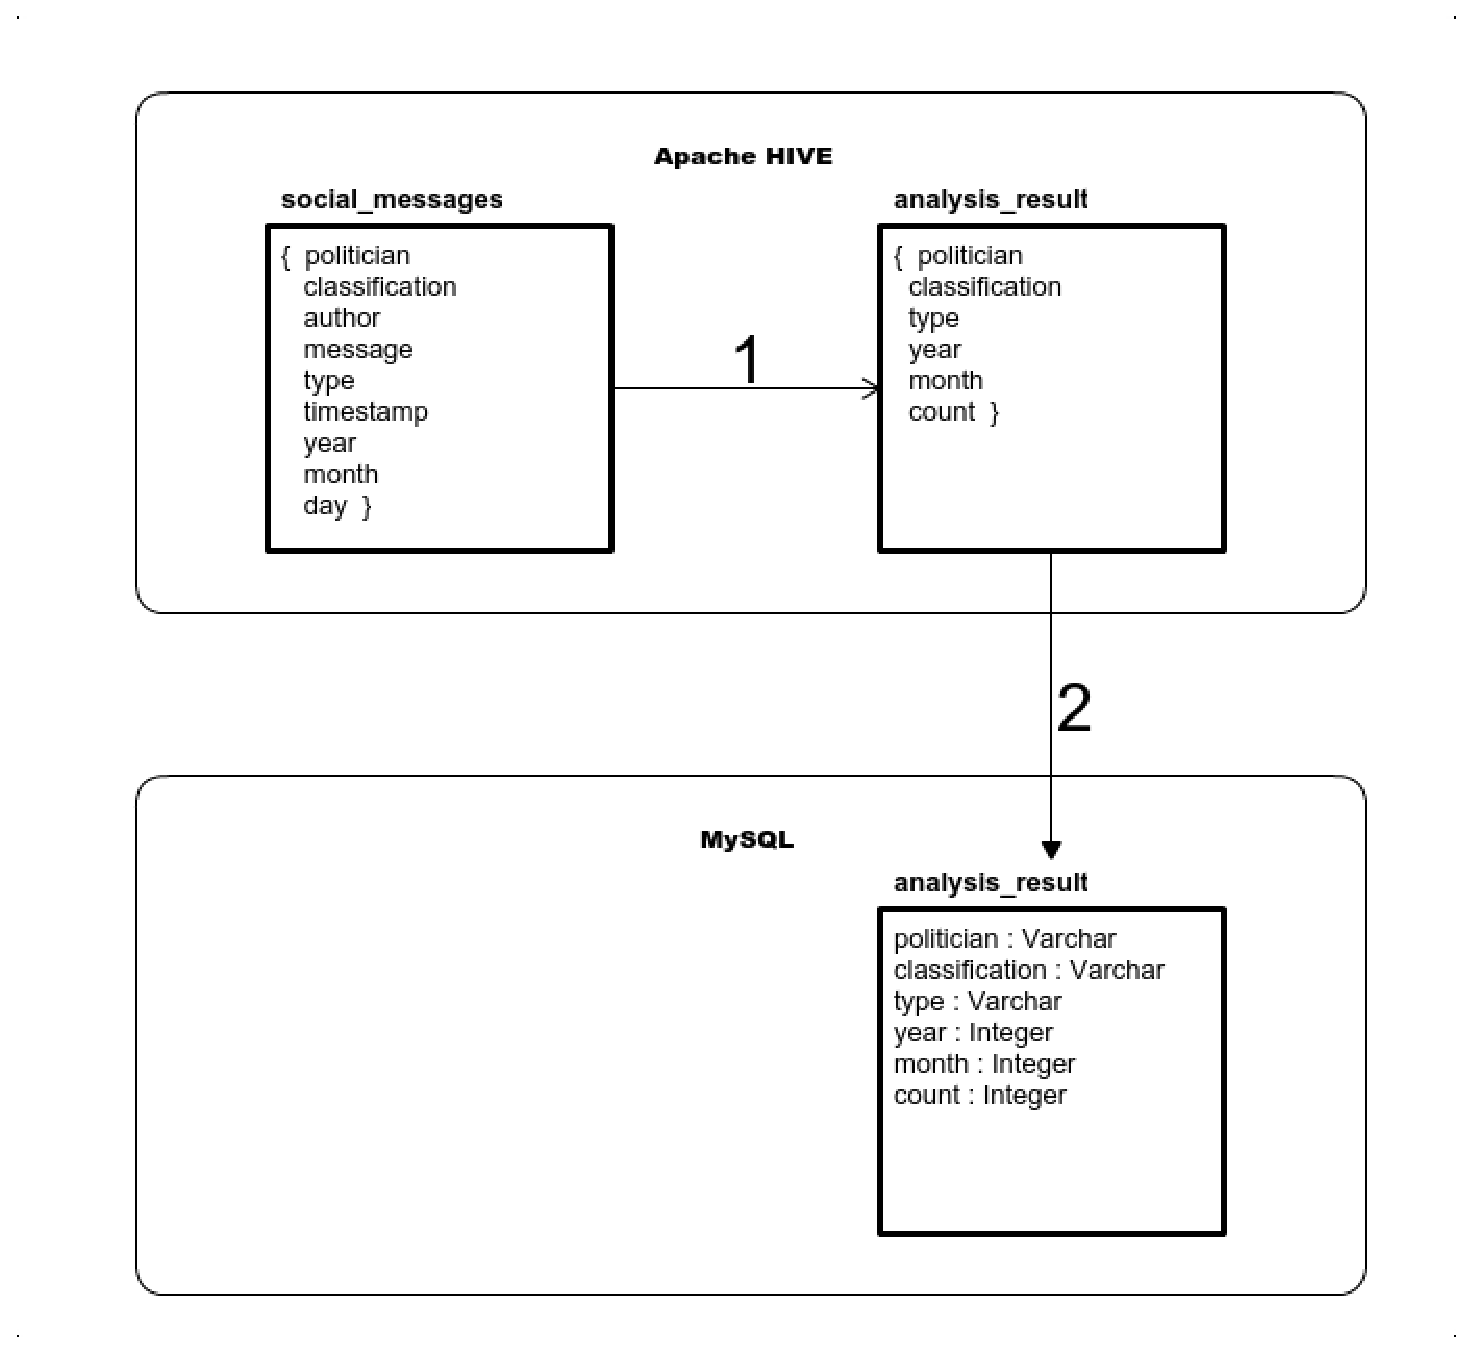
\includegraphics[keepaspectratio=true,scale=0.6]
	  {figuras/database.eps}
	\caption[Organização das tabelas]{Organização das tabelas
	\protect\linebreak Fonte: Autor}
	\label{tables}
\end{figure}
\FloatBarrier

A imagem \ref{tables} também representa o fluxo da informação até chegar ao MySQL. Inicialmente, a grande quantidade de mensagens persistidas na tabela \textit{social\_messages} são processadas e armazenadas em uma tabela intermediária no próprio Hive. A seta de número 1 indica a execução do comando HiveQL apresentado no quadro \ref{cod-load-analysis}. Através do Sqoop, representado pela seta de número 2, realiza-se a importação dos registros da tabela \textit{analysis\_result} para uma tabela idêntica, residente no MySQL. Com esta arquitetura, o Hive permite analisar informações em larga escala e de forma linear, enquanto o banco de dados relacional é usado para apresentar os resultados em tempo real.

\section{Exibição dos Resultados}

Nesta seção, será apresentada a última etapa do estudo de caso proposto por este trabalho. O objetivo desta fase é construir uma interface \textit{web} que apresente os resultados obtidos após a análise de sentimentos e processamento de todas as mensagens coletadas. Os requisitos deste componente podem ser expressos nos seguintes itens.

\begin{itemize}

  \item Apresentar a quantidade total de mensagens retiradas por cada uma das redes sociais usadas durante a etapa de busca por publicações.
  \item Apresentar graficamente os resultados da análise de sentimentos concluída sobre as mensagens dos candidatos observados.

\end{itemize}

A partir destas necessidades, se iniciou a fase de elaboração e implementação da aplicação. A construção deste componente foi feita com uso da linguagem de programação Java. Para auxílio no desenvolvimento \textit{web}, foi utilizado o \textit{framework} Vraptor\footnote{\url{http://www.vraptor.org/pt/}}, elaborado pela empresa Caelum\footnote{\url{https://www.caelum.com.br/}}. Uma das principais características desta desta tecnologia é o foco em alta produtividade e na simplicidade do código, onde o tempo para configurar a ferramenta e escrever códigos repetitivos são otimizados para que o desenvolvedor possa trabalhar especialmente na lógica do negócio. A alta curva de aprendizado e a clareza do código, facilitando a manutenção do sistema, também são atributos positivos deste modelo.

Ao contrario de paradigmas de desenvolvimento \textit{web} baseados em componentes, como JSF\footnote{\url{http://pt.wikipedia.org/wiki/JavaServer_Faces}}, o Vraptor é um \textit{framework} MVC\footnote{Padrão de projeto de software que separa a lógica da aplicação da interação do usuário com o sistema.} que trabalha de maneira \textit{RESTFul}, ou seja, é possível associar uma determinada \textit{URL} a um método de uma controladora, que posteriormente torna-se responsável por executar a lógica da aplicação. Uma das grandes vantagens desta tecnologia é a automatização da conversão de parâmetros da requisição HTTP em objetos esperados pela controladora, além da facilidade de controle da navegação das páginas.

Para o desenvolvimento da interface gráfica, utilizou-se o \textit{framework} Twitter \textit{Bootstrap}\footnote{\url{http://getbootstrap.com/}}. Este projeto \textit{open source} é uma das ferramentas mais conhecidas para customização e criação de páginas HTML. Para incluir o \textit{Bootstrap} no projeto, basta importar seus arquivos CSS\footnote{Mecanismo usado para adicionar estilos a documentos \textit{web} escritos em linguagem de marcação, como HTML ou XML.} e suas funções escritas em Javascript. Com isso, é possível usar seus componentes reutilizáveis e extensivos, permitindo o desenvolvimento de interfaces responsivas e estilizadas.

A imagem \ref{interface-uml} apresenta a arquitetura planejada para este módulo \textit{web}.

\begin{figure}[ht!]
	\centering
	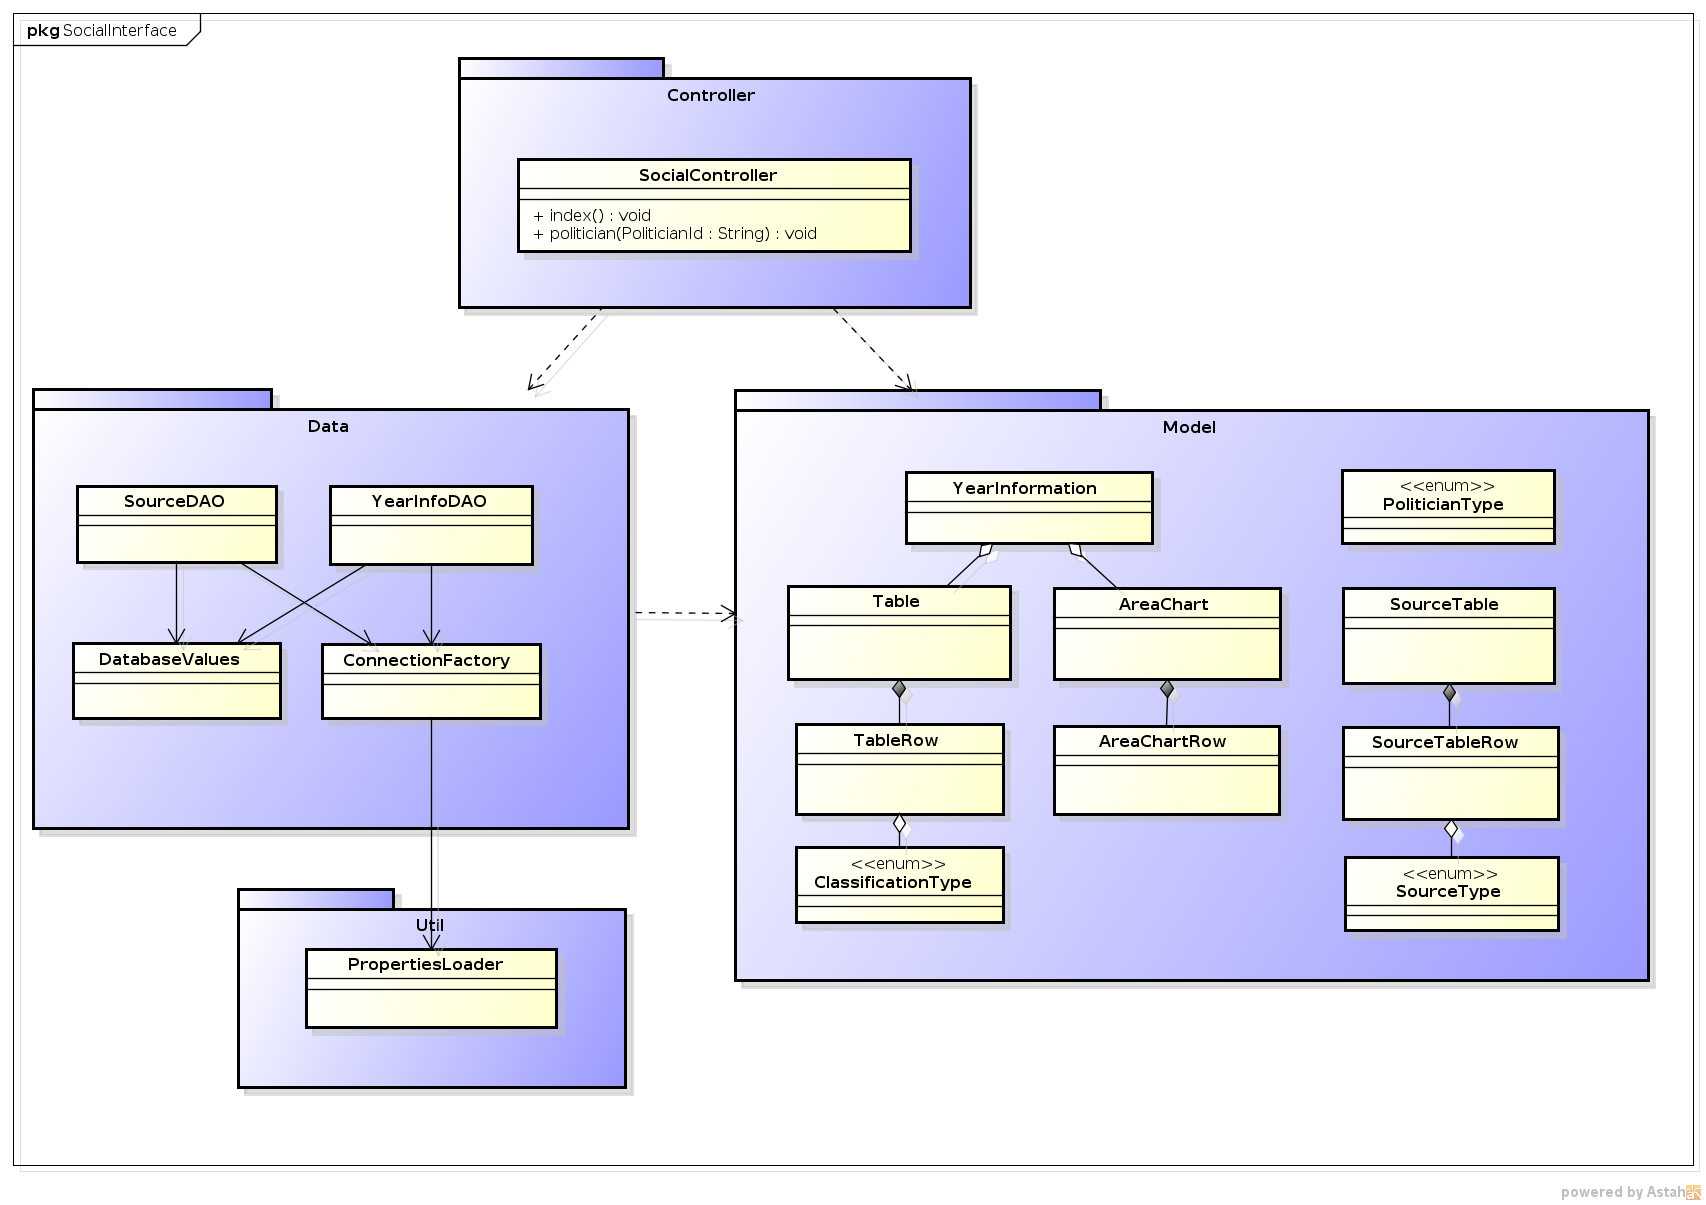
\includegraphics[keepaspectratio=true,scale=0.3]
	  {figuras/interface-uml.eps}
	\caption[Arquitetura da interface \textit{web}]{Arquitetura da interface \textit{web}
	\protect\linebreak Fonte: Autor}
	\label{interface-uml}
\end{figure}
\FloatBarrier

O pacote \textit{model} contém as classes de negócio, responsáveis por armazenar todas as informações que serão exibidas na interface gráfica. Já o pacote \textit{data}, engloba as classes que realizam consultas à tabela de resultados persistida no MySQL, além de converter estes dados para objetos do pacote \textit{model}. A classe \textit{PropertiesLoader} permite carregar as propriedades do banco de dados, que estão registradas em um arquivo físico no diretório raiz do projeto. Por fim, no pacote \textit{controller} está presente a controladora do Vraptor, responsável por gerenciar e responder as requisições feitas à aplicação.


